\section{Simplified Version} \label{simplified-version}

We begin by considering a simplified version of our survey. In this version,
there are just 17 complexity classes, and we will mostly examine their 
relationships in the world of all oracles.

\subsection{Complexity Classes}\label{class-definitions}

The classes in this mini-survey are listed here in alphabetical order, with
definitions for each.

\begin{itemize}
\item $\msf{ALL}$: The class of all languages. Naturally,
  $\msf{ALL}^f=\{\cL:\cL\subseteq\Sigma^*\}$ for every oracle $f$.
\item $\msf{AM}$: The class of languages computable by the \textit{Arthur-Merlin
    protocol}. Merlin is a \textit{prover} who wants to convince the
  \textit{verifier}, Arthur, that an input $x$ lies in the language
  $\cL$. Merlin knows at the outset whether $x\in\cL$ and can make any argument,
  but he is also biased: he wishes to convince Arthur that $x\in\cL$ regardless
  of whether this is actually true. Arthur, meanwhile, is a polynomial-time
  classical computer. Arthur may use randomness in his calculations, but the
  results of his coin tosses are known to Merlin in advance.

  A language $\cL$ is said to be in $\msf{AM}$ if, when $x\in\cL$, Merlin can
  convince Arthur of this fact with probability $\geq 2/3$, while if
  $x\not\in\cL$, then Merlin cannot convince Arthur that $x\in\cL$ with a
  probability of more than $1/3$. Formally, $\cL\in\msf{AM}^f$ if and only if 
  there exists a polynomial-time Turing machine $M$ with $f$-oracle and 
  functions $p(n),q(n)=\Oh(n^*)$ such that for every $x\in\Sigma^*$,
  \begin{align*}
    x\in\cL&\Longrightarrow\Pr_{y\in\Sigma^{p(|x|)}}[(\exists
    z\in\Sigma^{q(|x|)})[M(x,y,z)=1]]\geq 2/3, \\
    x\not\in\cL&\Longrightarrow\Pr_{y\in\Sigma^{p(|x|)}}[(\exists
    z\in\Sigma^{q(|x|)})[M(x,y,z)=1]]\leq 1/3.  
  \end{align*}
\item $\msf{BPP}$: The class of languages computable in polynomial time, with
  randomness. We can model $\msf{BPP}$ with a special probabilistic Turing
  machine capable of making coin tosses as part of its
  computation. Alternatively, we can make coin tosses in advance and supply the
  result to a deterministic Turing machine as an ancillary string along with
  the input. Formally, $\cL\in\msf{BPP}^f$ if and only if there exists a
  polynomial-time Turing machine $M$ with $f$-oracle and a function
  $p(n)=\Oh(n^*)$ such that for every $x\in\Sigma^*$,
  \[
  \Pr_{y\in\Sigma^{p(|x|)}}[M(x,y)=\cL(x)]\geq 2/3.
  \]
\item $\msf{BQP}$: The class of languages computable in polynomial time by a
  quantum computer. Formally, this means that languages in $\msf{BQP}$ are
  computable by a polynomially sized family of quantum circuits. As discussed in 
  Subsection \ref{quantum-model}, this family must be uniform.
\item $\msf{BQP}/\msf{qpoly}$: $\msf{BQP}$ with quantum polynomial advice. This 
  class consists of languages that can be computed by a polynomial-time quantum 
  computer with polynomial-length \textit{quantum advice}. Quantum advice is a 
  string of qubits that depends only on the length of the input; the qubits are 
  allowed to be in a state of superposition.
\item $\msf{EXP}$: The class of languages computable in
  exponential-time. Formally, $\cL\in\msf{EXP}^f$ if there exists an oracle
  Turing machine $M$ with $f$-oracle that computes $\cL$ in $T(n)$-time with
  $T(n)=\Oh(2^{p(n)})$, where $p(n)=\Oh(n^*)$.
\item $\msf{MA}$: The class of languages computable using the
  \textit{Merlin-Arthur protocol}. This is identical to the Arthur-Merlin
  protocol, except Arthur's coin tosses are unknown to Merlin. Formally,
  $\cL\in\msf{MA}^f$ if there exists a polynomial-time Turing machine $M$ with
  $f$-oracle and functions $p(n),q(n)=\Oh(n^*)$ such that for every $x\in\Sigma^*$,
  \begin{align*}
  x\in\cL&\Longrightarrow(\exists
  z\in\Sigma^{q(|x|)})\left[\Pr_{y\in\Sigma^{p(|x|)}}[M(x,y,z)=1]\geq
  2/3\right], \\
  x\not\in\cL&\Longrightarrow(\forall
  z\in\Sigma^{q(|x|)})\left[\Pr_{y\in\Sigma^{p(|x|)}}[M(x,y,z)=1]\leq 1/3\right].  
  \end{align*}
\item $\msf{NP}$: The class of languages that can be computed by a
  non-deterministic algorithm in polynomial-time. We replace the usual notion of
  a Turing machine with that of a non-deterministic Turing machine with two
  transition functions. Thus, instead of the computational process consisting of
  a sequence of configurations, it consists of a tree of configurations. Then
  $\cL\in\NP$ precisely when if $x\in\cL$, there is a path in the tree that
  accepts the input, while if $x\not\in\cL$, all paths reject. $\NP$ can also be
  defined using deterministic Turing machines with \textit{certificates}:
  formally, $\cL\in\NP^f$ if and only if there exist a polynomial-time oracle
  Turing machine $M$ with $f$-oracle and a function $p(n)=\Oh(n^*)$ such that for
  every $x\in\Sigma^*$,
  \[
  x\in\cL\Longleftrightarrow(\exists y\in\Sigma^{p(|x|)})[M(x,y)=1].
  \]
\item $\sP$: The class of languages that can be computed by a polynomial-time
  Turing machine (or an oracle Turing machine with $f$-oracle in the case of
  $\sP^f$). A polynomial-time Turing machine is one that, on an input of length
  $n$, terminates within $T(n)$ steps, where $T(n)=\Oh(n^*)$.
\item $\sP^{\#\sP}$: $\sP$ with $\#\sP$-oracle. This class consists of languages 
  computable in polynomial time with an oracle $f$ that lies in the function class 
  $\#\sP$. For a pair $(M,p)$ consisting of a polynomial-time Turing machine $M$ 
  and a function $p(n)=\Oh(n^*)$, set
  \[
  Y_{(M,p)}=\{y\in\Sigma^{p(|x|)}:M(x,y)=1\}.
  \]
  Then, $g:\Sigma^*\ra\Sigma^*$ lies in $\#\sP^f$ if and only if there exists a 
  pair $(M,p)$ such that $g(x)=|Y_{(M,p)}|$ for every $x\in\Sigma^*$. Now define 
  $(\sP^{\#\sP})^f=\bigcup_{g\in\#\sP^f}\sP^{g}$.
  
\item $\msf{PH}$: The polynomial hierarchy. For an oracle $f$, define
  $\Sigma_0\sP^f=\sP^f$. Then, for each $j\in\N$, set
  $\Sigma_{j+1}\sP^f=\NP^{\Sigma_j\sP^f}$. Finally, define
  $\msf{PH}=\bigcup_{j=0}^\infty\Sigma_j\sP^f$. We also define $\Pi_j\sP^f$ and
  $\Delta_j\sP^f$ by $\Sigma_0\sP^f=\Delta_0\sP^f=\sP^f$ and
  $\Pi_j\sP^f=\co\NP^{\Sigma_{j-1}\sP^f}$,
  $\Delta_j\sP^f=\sP^{\Sigma_{j-1}\sP^f}$ for $j\geq 1$.
\item $\msf{PP}$: Like $\msf{BPP}$, a class of polynomial-time computable
  languages, with randomness. The defining condition of $\msf{PP}$ is weaker
  than that of $\msf{BPP}$, requiring only that if an input $x$ lies in the
  language, a probabilistic Turing machine obtains the correct answer with a
  probability of at least $1/2$. Formally, $\cL\in\msf{PP}^f$ if and only if
  there exists a polynomial-time Turing machine $M$ with $f$-oracle and a
  function $p(n)=\Oh(n^*)$ such that for every $x\in\Sigma^*$,
  \[
  x\in\cL\Longleftrightarrow\Pr_{y\in\Sigma^{p(|x|)}}[M(x,y)=1]\geq 1/2.
  \]
\item $\sP/\msf{poly}$: $\sP$ with polynomial advice. An \textit{advice string}
  is a fixed string $y_n$ that accompanies an input of length $n$. Being
  \textit{polynomial} advice means that the function $n\mapsto|y_n|$ is
  $\Oh(n^*)$. Formally, $\cL\in(\sP/\poly)^f$ if and only if there exist a
  polynomial-time oracle Turing machine $M$ with $f$-oracle and a function
  $g:\N\mapsto\Sigma^*$, where $|g(n)|=\Oh(n^*)$, such that for every
  $x\in\Sigma^*$,
  \[
  x\in\cL\Longleftrightarrow M(x,g(|x|))=1.
  \]
  Equivalently, $\sP/\poly$ is the class of languages that can be computed by a 
  non-uniform family of polynomial-size classical circuits (see Subsection 
  \ref{classical-models}).
\item $\msf{PSPACE}$: The class of languages that are polynomial-space
  computable. For a function $T:\N\ra\N$, $\cL\in\msf{SPACE}(T(n))^f$ if and
  only if there exist an oracle Turing machine $M$ with $f$-oracle that computes
  $\cL$ and a constant $C$ such that, when $x\in\Sigma^*$ is given as an input
  to the machine, there are at most $CT(|x|)$ cells of each tape that are ever
  written onto during the computation. Then, define
  $\msf{PSPACE}^f=\bigcup_{k=0}^\infty\msf{SPACE}(n^k)^f$. We adopt the convention
  that the space limitation of $\msf{PSPACE}^f$ applies to the oracle tape as 
  well, so that oracle calls are limited to a polynomial of the length of the
  input.
\item $\msf{QAM}$: The class of languages using the quantum 
  Arthur-Merlin protocol. The definition is similar to $\msf{AM}^f$, except $M$ is 
  a polynomial-time quantum computer with $f$-oracle rather than a classical 
  computer, and Merlin is an all-powerful quantum-computer capable of computing any
  system of qubits. Arthur sends Merlin a random string of classical bits, Merlin 
  responds with a polynomial-length quantum message, and then Arthur uses the 
  random bits along with Merlin's message to decide whether to accept or reject the
  input.
\item $\msf{QMA}$: The class of languages using the quantum Merlin-Arthur
  protocol. The definition is the same as $\msf{MA}^f$, except $M$ is a
  polynomial-time quantum computer with $f$-oracle rather than a classical
  computer, and Merlin is an all-powerful quantum-computer. Arthur and Merlin 
  exchange messages in the form of systems of qubits rather than classical bit 
  strings.
\item $\msf{SZK}$: Traditionally defined as the class of languages that can be 
  computed using a statistical zero-knowledge proof protocol, $\msf{SZK}$ can be 
  defined in a simpler way using a special case of this protocol. We call the 
  special case the \textit{rhetorical question protocol}. This is 
  similar to the Arthur-Merlin protocol, except that Arthur's message to Merlin 
  consists of a question for which Arthur has privately computed a correct answer. 
  Arthur accepts the input if and only if Merlin's 
  response matches Arthur's correct answer. Formally, $\cL\in\msf{SZK}^f$ if and 
  only if there exist a polynomial-time oracle Turing machine $M$ with $f$-oracle 
  and a function $p(n)=\Oh(n^*)$ such that for all $x\in\Sigma^*$,
  \begin{align*}
  x\in\cL&\Longrightarrow(\exists P\in\mathcal{M})
  \left[\Pr_{y\in\Sigma^{p(|x|)}}[P(x,M(x,y,0))=M(x,y,1)]\geq 2/3\right], \\
  x\not\in\cL&\Longrightarrow(\forall P\in\mathcal{M})
  \left[\Pr_{y\in\Sigma^{p(|x|)}}[P(x,M(x,y,0))=M(x,y,1)]\leq 1/3\right],
  \end{align*}
  where
  \[
  \mathcal{M}=
  \{P:\Sigma^*\ra\Sigma^*:(\exists q(n)=\Oh(n^*))[P(x)\in\Sigma^{q(|x|)}]\}.
  \]
  See Subsection \ref{szk-subsection} for a discussion of the relationship between 
  this definition of $\msf{SZK}$ and a more conventional definition.
\end{itemize}

\subsection{Inclusions}

To establish the overall structure of the relationships between these 17
complexity classes, we first establish which inclusions are relativizing --
i.e., which inclusions hold for every oracle. To that end, we identify the
symmetric classes, by which we mean the classes $\sC$ such that
$\sC=\cco\cdot\sC$ with respect to every oracle. This will allow us to easily
strengthen many of the inclusions described here. For example, knowing that
$\sP$ is symmetric and that $\sP\subseteq\NP$ for every oracle allows us to
conclude that $\sP\subseteq\cocap\cdot\NP=\NP\cap\co\NP$ with respect to every
oracle.

It is immediate that $\sP$ is symmetric, because a polynomial-time computer can
simply swap its output $\alpha$ with $1-\alpha$. The computer can still perform
this operation if it is quantum, exponential-time, polynomial-space, or has
access to a $\#\sP$-oracle, so $\msf{BQP}$, $\msf{EXP}$, $\msf{PSPACE}$, and
$\sP^{\#\sP}$ are likewise symmetric. A computer receiving advice strings does
not affect this capacity, so $\sP/\poly$ and $\msf{BQP}/\poly$ are symmetric as
well. As was shown in Section \ref{operator-section}, the operators $\cBP$
and $\cP$ commute with $\cco$. Since $\msf{BPP}=\cBP\cdot\sP$ and
$\msf{PP}=\cP\cdot\sP$, it follows that $\msf{BPP}$ and $\msf{PP}$ are
symmetric. Of course, $\msf{ALL}$ is clearly symmetric.

$\msf{PH}$ is symmetric, because $\msf{PH}=\bigcup_{k=0}^\infty\Sigma_k\sP=\bigcup_{k=0}^\infty\Pi_k\sP$. More explicitly:
\begin{lemma}
For every $k\in\N$, $\Delta_k\sP\subseteq\Sigma_k\sP$,
$\Delta_k\sP\subseteq\Pi_k\sP$, $\Sigma_k\sP\subseteq\Delta_{k+1}\sP$, and
$\Pi_k\sP\subseteq\Delta_{k+1}\sP$.
\end{lemma}

\begin{proof}
In the case that $k=0$, $\Delta_k\sP\subseteq\Sigma_k\sP$ because both classes
are equal to $\sP$. If $k>0$, then
$\Delta_k\sP\subseteq\sP^{\Sigma_{k-1}\sP}\subseteq\NP^{\Sigma_{k-1}\sP}=\Sigma_k\sP$.
Since $\Delta_k\sP$ is a symmetric class (being $\sP$ with an oracle), it
follows that $\Delta_k\sP\subseteq\Pi_k\sP$ for every $k$.

For the second pair of inclusions,
$\Delta_k\sP\subseteq\sP^{\Sigma_k\sP}=\Delta_{k+1}\sP$, and then
$\Pi_k\sP\subseteq\Delta_{k+1}\sP$ likewise follows from the symmetry of
$\Delta_{k+1}\sP$.
\end{proof}

$\msf{SZK}$ is a symmetric class:

\begin{theorem}[Okamoto, \cite{okamoto2000relationships}]
$\msf{SZK}=\cco\cdot\msf{SZK}$ with respect to any oracle.
\end{theorem}

Next we discuss which complexity classes are subsets of each other relative to
every oracle. We consider a minimal generating set of inclusions, which in this
context means that all the inclusions will be Hasse relative to the 17 classes
we are considering. In other words, we do not need to prove
$\sP\subseteq\msf{MA}$ because this follows from $\sP\subseteq\NP$ and
$\NP\subseteq\msf{MA}$.

$\sP\subseteq\msf{BPP}$ and $\sP\subseteq\msf{NP}$ are true because both
$\msf{BPP}$ and $\msf{NP}$ are polynomial-time classes, but with additional
powers that can be ignored: to simulate $\sP$ with $\msf{BPP}$, make no coin
tosses; to simulate $\sP$ with $\msf{NP}$, discard the certificate.
Alternatively both inclusions can be said to follow from the properties in
Section \ref{operator-section}, since $\msf{BPP}=\cBP\cdot\sP$ and
$\msf{NP}=\cN\cdot\sP$. Similarly, 
$\msf{BQP}\subseteq\msf{BQP}/\msf{qpoly}$.

As was mentioned during the discussion on the pseudo-operator $\mathpzc{Q}$ in
Section \ref{operator-section}, a quantum computer can perform the same
operations as a classical computer (possibly with the aid of ancilliary qubits).
This applies to probabilistic classic computers as well as deterministic ones,
because a coin flip can be simulated by measuring the qubit
$\frac{1}{\sqrt{2}}(\ket{0}+\ket{1})$. Hence $\msf{BPP}\subseteq\msf{BQP}$. By 
the same principle, $\sP/\poly\subseteq\msf{BQP}/\msf{qpoly}$, 
$\msf{MA}\subseteq\msf{QMA}$, and $\msf{AM}\subseteq\msf{QAM}$.

The inclusion $\msf{BPP}\subseteq\msf{MA}$
is straightforward: in the definition of $\msf{MA}$, the
verifier is a probabilistic polynomial-time Turing machine that must reach the
correct answer with a probability of at least $2/3$. Thus, a protocol in which
Arthur ignores the Merlin and performs his own computations is an
an $\msf{MA}$-protocol that computes a problem in
$\msf{BPP}$. The same argument also shows that $\msf{BQP}\subseteq\msf{QMA}$. 
Similarly, $\msf{BPP}\subseteq\msf{SZK}$. While our definition of $\msf{SZK}$ 
requires that Arthur bases his conclusion on the response given by Merlin, Arthur 
can effectively ``ignore'' Merlin by either telling Merlin the correct answer (if 
Arthur wants to accept the input) or generating a random string as the correct 
answer and sending a blank message to Merlin (if Arthur wants to reject the input).

$\msf{BPP}$ can be \textit{derandomized}, allowing it to be placed inside
$\sP/\poly$.

\begin{theorem}[Adleman, \cite{adleman1978two}]
$\msf{BPP}\subseteq\sP/\poly$ relative to every oracle.
\end{theorem}

\begin{proof}
Let $\cL\in\msf{BPP}$. The class $\msf{BPP}$ is subject to an error-reducing
procedure: by running several copies of a $\msf{BPP}$-machine in parallel and
taking the ``majority vote'' of the machines, we can obtain the correct answer
with a higher probability. Using this technique, we can suppose that there
exists a polynomial-time Turing machine $M$ and a function $p(n)=\Oh(n^*)$ such
that for every $x\in\Sigma^*$,
\[
\Pr_{y\in p(|x|)}[M(x,y)\neq\cL(x)]\leq 1/2^{|x|+1}.
\]
Equivalently, for every $x\in\Sigma^*$ there are at most $2^{p(|x|)-|x|-1}$ 
strings $y\in\Sigma^{p(|x|)}$ such that $M(x,y)\neq\cL(x)$. For $x\in\Sigma^*$, 
set
\[
B_x=\{y\in\Sigma^{p(|x|)}:M(x,y)\neq\cL(x)\},
\]
and for $n\in\N$, set
\[
B_n=\bigcup_{x\in\Sigma^n}B_x.
\]
$B_n$ is the set of ``bad advice'' for an input of length $n$. Now
\[
|B_n|\leq\Sigma_{|x|=n}|B_x|\leq\Sigma_{|x|=n}2^{p(n)-n-1}=2^n2^{p(n)-n-1}=
2^{p(n)-1}<2^{p(n)}=|\Sigma^{p(n)}|,
\]
so the set $\Sigma^{p(n)}\setminus B_n$ is nonempty for every $n$. Thus, there
exists a function $f:\N\ra\Sigma^*$ such that $f(n)\in\Sigma^{p(n)}\setminus
B_n$ for every $n$. We therefore have that for each $x\in\Sigma^*$,
\[
M(x,f(|x|))=\cL(x),
\]
so $\cL\in\sP/\poly$ as desired.
\end{proof}

The fact $\NP\subseteq\msf{MA}$ follows from the observation that replacing the 
definition of $MA$ with a deterministic Turing machine is precisely the 
definition of $\NP$.

We now consider the relationship between $\msf{AM}$ and $\msf{MA}$. To do this, 
we indroduce related (and seemingly different) classes $\msf{AM}[k]$ for 
integers $k\geq 2$. This represents the Arthur-Merlin protocol with $k$ rounds.

\begin{definition}
A $k$-round Arthur-Merlin protocol is an interaction $(V,P)_k$ between a 
probabilistic Turing machine $V$, representing Arthur, and a function 
$P:\Sigma^*\ra\Sigma^*$, representing Merlin. Given an input $x\in\Sigma^*$, 
Arthur computes a message $m_1$ and sends it, along with the random bits $y_1$ 
used in the computation, as a string $\alpha_1=\inner{m_1,y_1}$ to Merlin. 
Merlin responds with a string $\alpha_2$ that is limited in length by a 
polynomial in $|x|$. Arthur sends a new message $\alpha_3=\inner{m_3,y_3}$, 
Merlin responds with $\alpha_4$, and so on, until the sequence 
$(\alpha_1,\ldots,\alpha_k)$ has been generated. Then Arthur deterministically 
computes $V(\alpha_1,\ldots,\alpha_k)$ to decide whether to accept the input. 
We denote the result by $\out_{(V,P)_k}(x)$.

A language $\cL$ lies in $\msf{AM}[k]$ if and only if there exists a 
polynomial-time Turing machine $V$ such that for every $x\in\Sigma^*$,
\begin{align*}
x\in\cL&\Longrightarrow
(\exists P\in\mathcal{M})\Pr[\out_{(V,P)_k}(x)=1]\geq 2/3, \\
x\not\in\cL&\Longrightarrow
(\forall P\in\mathcal{M})\Pr[\out_{(V,P)_k}(x)=1]\leq 1/3,
\end{align*}
where
\[
\mathcal{M}=\{P:\Sigma^*\rightarrow\Sigma^*:(\exists 
q(n)=\Oh(n^*))[P(x)\in\Sigma^{q(|x|)}]\}.
\]
\end{definition}
With this definition, we obtain $\msf{AM}=\msf{AM}[2]$. Moreover, Arthur can 
imitate the Merlin-Arthur protocol within a 3-round Arthur-Merlin protocol: 
after sending his message to Merlin and receiving a response, Arthur makes his 
final computation with a fresh set of random bits. These bits are sent to 
Merlin, but since Merlin cannot send a second response, these random bits are 
effectively private. Hence $\msf{MA}\subseteq\msf{AM}[3]$.

As it turns out, however, adding extra rounds to an Arthur-Merlin protocol does 
not change the computational power of $\msf{AM}$:
\begin{theorem}[Babai, \cite{babai1985trading}]
$\msf{AM}[k+1]\subseteq\msf{AM}[k]$ with respect to any oracle for all integers 
$k\geq 2$.
\end{theorem}
$\msf{AM}[2]\subseteq\msf{AM}[3]\subseteq\msf{AM}[4]\subseteq\ldots$, since Arthur 
can choose to ignore the later rounds of his interaction with Merlin. Hence 
$\msf{AM}=\msf{AM}[k]$ for every $k$.

As an immediate corollary of $\msf{MA}\subseteq\msf{AM}[3]$ and the above 
theorem, we deduce $\msf{MA}\subseteq\msf{AM}$. These arguments are not 
affected if Arthur is quantum rather than classical, so we also have 
$\msf{QMA}\subseteq\msf{QAM}$. Okamoto \cite{okamoto2000relationships} showed that 
$\msf{SZK}$ could be characterized by a constant-round protocol with a public-coin 
Arthur; it follows that $\msf{SZK}\subseteq\msf{AM}$.

To see that $\msf{AM}\subseteq\msf{PH}$, we need an alternate characterization 
of $\msf{PH}$:
\begin{lemma}
For every language $\cL\subseteq\Sigma^*$, $\cL\in\Sigma_k\sP$ if and only if 
there exists a polynomial-time Turing machine $M$ and 
$p_1(n),\ldots,p_k(n)=\Oh(n^*)$ such that for all $x\in\Sigma^*$,
\[
x\in\cL\Longleftrightarrow
(Q_1 y_1\in p_1(|x|))\ldots(Q_k y_k\in p_k(|x|))
[M(x,y_1,\ldots,y_k)=1],
\]
where $Q_j$ is $\exists$ when $j$ is odd and $\forall$ when $j$ is even.
\end{lemma}
\begin{proof}
Denote this alternative version of $\Sigma_k\sP$ by $\bar\Sigma_k\sP$, and 
denote $\bar\Pi_n\sP=\cco\cdot\bar\Sigma_k\sP$. If $k=0$, then 
$\Sigma_0\sP=\bar\Sigma_0\sP=\sP$. Thus, we can suppose for induction that 
$\Sigma_{k+1}\sP=\bar\Sigma_{k+1}\sP$. We have
\[
\bar\Sigma_{k+1}\sP=\cN\cdot\bar\Pi_k\sP=\cN\cdot\Pi_k\sP\subseteq
\cN\cdot\sP^{\Pi_k\sP}=\cN\cdot\sP^{\Sigma_k\sP}=\NP^{\Sigma_k\sP}=
\Sigma_{k+1}\sP,
\]
so it suffices to show that $\Sigma_{k+1}\sP\subseteq\bar\Sigma_{k+1}\sP$.

Suppose $\cL\in\Sigma_{k+1}\sP$. Then there exists a polynomial-time Turing 
machine $M$ with $f$-oracle, where $f\in\Sigma_k\sP$, and a function 
$p(n)=\Oh(n^*)$ such that
\begin{equation}\label{PH1}
x\in\cL\Longleftrightarrow
(\exists y\in\Sigma^{p(|x|)})[M(x,y)=1]
\end{equation}
for every $x\in\Sigma^*$. On an input $\inner{x,y}$, the machine makes $q(|x|)$ 
oracle calls, where $q(n)=\Oh(n^*)$. Let $M^\prime$ be the polynomial-time Turing 
machine such that $M^\prime(x,y,a_1,\ldots,a_{q(|x|)})$ computes $M(x,y)$ when 
$a_1,\ldots,a_{q(|x|)}$ are given as oracle replies. Then (\ref{PH1}) can be 
written as 
\begin{equation}
x\in\cL\Longleftrightarrow
(\exists y\in\Sigma^{p(|x|)},a_1,\ldots,a_{q(|x|)}\in\Sigma^{q(|x|)})
[M^\prime(x,y,a_1,\ldots,a_{q(|x|)})\AND a_1,\ldots,a_{q(|x|)}\text{ are 
correct}].
\end{equation}\label{PH2}
"Correct" means that, if $M$ queries the oracle with $z$, the oracle responds 
with $f(z)$. It is enough to show that ``$a_1,\ldots,a_{q(|x|)}$ are correct'' 
is a $\bar\Sigma_{k+1}\sP$ predicate, because then the entire right side of 
(\ref{PH2}) is a $\bar\Sigma_{k+1}\sP$ predicate. To see that this is the case, 
note that given $x$, $y$, and $a_1,\ldots,a_{q(|x|)}$, we can complete the 
queries $z_1,\ldots,z_{q(|x|)}$ given to the oracle in polynomial time (let 
$M^\prime$ run, and then record the oracle queries as they occur). Then 
``$a_1,\ldots,a_{q(|x|)}$ are correct'' is equivalent to
\[
\bigwedge_{j=1}^{q(|x|)}[A(z_j)=a_j],
\]
which is a conjunction of $\Oh(|x|^*)$-many $\bar\Sigma_{k+1}\sP$ predicates 
(specifically, $(z_j)=1$ is a $\bar\Sigma_k$ predicate, and $f(z_j)=0$ is a 
$\bar\Pi_k$ predicate) and therefore a $\bar\Sigma_{k+1}\sP$ predicate itself. 
Hence $\cL\in\bar\Sigma_{k+1}\sP$ as desired.
\end{proof}
We also need the following result:
\begin{theorem}[Sipser-G\`acs-Lautemann]
If $\cL\in\cBP\cdot\sC$ for a complexity class $\sC$, there exist
$\cL^\prime\in\sC$ and functions $p(n),q(n)=\Oh(n^*)$ such that
\[
x\in\cL\Longleftrightarrow
(\exists u_1,\ldots, u_{p(|x|)}\in\Sigma^{q(|x|)})
(\forall r\in\Sigma^{q(|x|)})
\left[\bigvee_{j=1}^{p(|x|)}\inner{x,r+_2u_j}\in\cL^\prime\right],
\]
where $+_2$ denotes entrywise addition modulo 2.
\end{theorem}
\begin{proof}
Let $\cL\in\cBP\cdot\sC$. By the same error-reduction procedure used in the
proof of $\msf{BPP}\subseteq\sP/\poly$, there exists a language 
$\cL^\prime\in\sC$ and a function $p(n)=\Oh(n^*)$ such that for every 
$x\in\Sigma^*$,
\begin{align}
\label{SGL1} x\in\cL&\Longrightarrow
\Pr_{y\in\Sigma^{p(|x|)}}[\inner{x,y}\in\cL^\prime]\geq 1-2^{-|x|}, \\ 
\label{SGL2} x\not\in\cL&\Longrightarrow
\Pr_{y\in\Sigma^{p(|x|)}}[\inner{x,y}\in\cL^\prime]\leq 2^{-|x|}. 
\end{align}
For each $x\in\Sigma^*$, set
\[
A_x=\{y\in\Sigma^{p(|x|)}:\inner{x,y}\in\cL^\prime\}.
\]
Then (\ref{SGL1}) and (\ref{SGL2}) can be rewritten as
\begin{align}
\label{SGL1P} x\in\cL&\Longrightarrow
|A_x|\geq 2^{p(|x|)}(1-2^{-|x|}), \\ 
\label{SGL2P} x\not\in\cL&\Longrightarrow
|A_x|\leq 2^{p(|x|)-|x|}.
\end{align}
Now for $m\in\N$, $S\subseteq\Sigma^m$, and $u\in\Sigma^m$, set
\[
S+_2u=\{y+_2u:y\in S\}.
\]
Note that for any $n\in\N$, if $S\subseteq\Sigma^{p(n)}$ satisfies $|S|\leq 
2^{p(n)-n}$, then for any $u_1,\ldots,u_k\in\Sigma^{p(n)}$ with $k<2^n$, we have
\[
\left|\bigcup_{j=1}^k(S+_2u_j)\right|\leq
\sum_{j=1}^k|S+_2u_j|=k|S|\leq k2^{p(n)-n}<2^{p(n)},
\]
so that $\bigcup_{j=1}^k(S+_2u_j)\neq\Sigma^{p(|x|)}$. In particular, if we set 
$q(n)=\lceil p(n)/n)\rceil+1$ for every $n\in\N$ (we will need the fact that 
$p(n)<nq(n)$ shortly), then it follows from 
(\ref{SGL2P}) that
\begin{equation}\label{SGL3}
x\not\in\cL\Longrightarrow
(\forall u_1,\ldots,u_{q(|x|)}\in\Sigma^{p(|x|)})
\left[\bigcup_{j=1}^{q(|x|)}(A_x+_2u_j)\neq\Sigma^{p(|x|)}\right].
\end{equation}
On the other hand, suppose that $S\subseteq\Sigma^{p(|x|)}$ satisfies 
$|S|\geq 2^{p(n)}(1-2^{-n})$. Let $u_1,\ldots,u_{q(n)}\in\Sigma^{p(n)}$ be 
chosen uniformly randomly. Then $r+_2u_j$ is also randomly chosen for any 
partucular $r$, and we can compute as follows:
\begin{align*}
\Pr\left[\bigcup_{j=1}^{q(n)}(S+_2u_j)\neq\Sigma^{p(n)}\right]
&=\Pr\left[(\exists r\in\Sigma^{p(n)})\left[r\not\in\bigcup_{j=1}^{q(n)}
(S+_2u_j)\right]\right] \\
&=\Pr\left[(\exists r\in\Sigma^{p(n)})\left[\bigvee_{j=1}^{q(n)}r\not\in
S+_2u_j\right]\right] \\
&=\Pr\left[(\exists r\in\Sigma^{p(n)})\left[\bigvee_{j=1}^{q(n)}r+_2u_j\not\in
S\right]\right] \\
&=\Pr\left[\bigvee_{j=1}^{q(n)}u_j\not\in S\right]
=\prod_{j=1}^{q(n)}\Pr[u_j\not\in S]
\leq\prod_{j=1}^{q(n)}2^{-n}
=2^{-nq(n)}<2^{-p(n)}<1.
\end{align*}
Hence $\Pr[\bigcup_{j=1}^{q(n)}(S+_2u_j)=\Sigma^{p(n)}]>0$, and so it follows 
from (\ref{SGL1P}) that
\begin{equation} \label{SGL4}
x\in\cL\Longrightarrow(\exists u_1,\ldots,u_{q(|x|)}\in\Sigma^{p(|x|)})
\left[\bigcup_{j=1}^{q(|x|)}(A_x+u_j)=\Sigma^{p(|x|)}\right].
\end{equation}
(\ref{SGL3}) and (\ref{SGL4}) together are equivalent to the desired result.
\end{proof}
\begin{corollary}
$\msf{AM}\subseteq\Pi_2\sP$ with respect to every oracle.
\end{corollary}
\begin{proof}
The definition of $\msf{AM}$ gives $\msf{AM}=\cBP\cdot\NP$ and hence 
$\cco\cdot\msf{AM}=\cBP\cdot\co\NP$. Thus, by the previous theorem, for 
$\cL\in\cco\cdot\msf{AM}$ there exist $\cL^\prime\in\co\NP$ and 
$p(n),q(n)=\Oh(n^*)$ such that
\[
x\in\cL\Longleftrightarrow
(\exists u_1,\ldots, u_{p(|x|)}\in\Sigma^{q(|x|)})
(\forall r\in\Sigma^{q(|x|)})
\left[\bigvee_{j=1}^{p(|x|)}\inner{x,r+_2u_j}\in\cL^\prime\right]
\]
for every $x\in\Sigma^*$. It follows that $\cL\in\Sigma_2\sP$ by the quantifier 
definition of $\Sigma_2\sP$. Therefore, $\cco\cdot\msf{AM}\subseteq\Sigma_2\sP$.
\end{proof}
We next have $\msf{QMA}\subseteq\msf{PP}$ \cite{vyalyi2003qma} with respect to 
every oracle. In fact, $\msf{QMA}\subseteq\msf{A}_0\msf{PP}$, where 
$\msf{A}_0\msf{PP}\subseteq\msf{PP}$ is a class defined as follows: for 
$\cL\subseteq\Sigma^*$, we say $\cL\in\msf{A}_0\msf{PP}$ if and only if there 
exist functions $f,g:\Sigma^*\ra\Sigma^*$, where $g$ is polynomial-time 
computable and
\[
f(x)=|\{y\in\Sigma^{p(|x|)}:M(x,y)=1\}|-|\{y\in\Sigma^{p(|x|)}:M(x,y)=0\}|
\]
for a polynomial-time Turing machine $M$ and $p(n)=\Oh(n^*)$, such that for every 
$x\in\Sigma^*$,
\begin{align*}
x\in\cL&\Longrightarrow f(x)>g(x), \\
x\not\in\cL&\Longrightarrow f(x)<g(x)/2.
\end{align*}
We now consider the class $\sP^{\#\sP}$. $\#\sP$ can be considered to be 
the function class analogue of $\msf{PP}$ in the same way that $\msf{FP}$, the 
class of polynomial-time computable functions, is the function class analogue 
of $\sP$. In general, including a $\sP$-oracle in a computational process is 
equivalent to including an $\msf{FP}$-oracle, because with a $\sP$-oracle one 
can determine the output $f(x)$ of a function $f\in\msf{FP}$ by successively 
computing each bit of $f(x)$. Similarly, a $\msf{PP}$-oracle can be used to 
determine each bit of the output of a function in $\#\sP$, thereby simulating a 
$\#\sP$-oracle. Hence $\sP^{\#\sP}=\sP^{\msf{PP}}$. It follows that 
$\msf{PP}\subseteq\sP^{\#\sP}$ (this only requires the straightforward direction
$\sP^{\msf{PP}}\subseteq\sP^{\#\sP}$).

$\sP^{\#\sP}$ also contains the polynomial hierarchy:
\begin{theorem}[Toda, \cite{toda1991pp}]
$\msf{PH}\subseteq\sP^{\#\sP}$ relative to every oracle.
\end{theorem}
Another inclusion that makes use of an intermediate class is 
$\msf{QAM}\subseteq\msf{PSPACE}$.
\begin{theorem}[\cite{marriott2005quantum}]
$\msf{QAM}\subseteq\cBP\cdot\msf{PP}$ relative to every oracle.
\end{theorem}
Now $\cBP\cdot\msf{PP}\subseteq\msf{PSPACE}$.
\begin{lemma}
$\msf{PP}\subseteq\msf{PSPACE}$.
\end{lemma}
\begin{proof}
Since $\msf{PSPACE}$ is not limited in computational time, given a 
polynomial-time Turing machine $M$ and a function $p(n)=\Oh(n^*)$, a 
$\msf{PSPACE}$-machine can simulate a $\msf{PP}$-machine by keeping a tally of 
how many $y\in\Sigma^{p(|x|)}$ satisfy $M(x,y)=1$ for the input $x$.
\end{proof}
This derandomization also applies to the probabilistic version of 
$\msf{PSPACE}$.
\begin{lemma}
$\cBP\cdot\msf{PSPACE}\subseteq\msf{PSPACE}$.
\end{lemma}
It now follows that
\[
\msf{QAM}\subseteq\cBP\cdot\msf{PP}\subseteq\cBP\cdot\msf{PSPACE}\subseteq
\msf{PSPACE}.
\]
With one additional lemma, we can also prove that 
$\sP^{\#\sP}\subseteq\msf{PSPACE}$.
\begin{lemma}
If $\cL\in\msf{PSPACE}$, then $\msf{PSPACE}^\cL\subseteq\msf{PSPACE}$.
\end{lemma}
\begin{proof}
By our convention, oracle calls are limited in length to a polynomial of the imput.
Hence any calls to the oracle in a $\msf{PSPACE}^\cL$-machine can be replaced with 
a direct computation of $\cL(x)$ by a $\msf{PSPACE}$-machine.
\end{proof}
Now
\[
\sP^{\#\sP}\subseteq\sP^{\msf{PP}}\subseteq\msf{PSPACE}^{\msf{PSPACE}}\subseteq
\msf{PSPACE}.
\]
For our final $\msf{PSPACE}$ inclusion, observe that a $\msf{PSPACE}$-machine is
limited to $2^{p(n)}$ possible configurations for an input of length $n$, where 
$p(n)=\Oh(n^*)$. Thus, any computation that halts must do so within $2^{p(n)}$ 
steps. Therefore $\msf{PSPACE}\subseteq\msf{EXP}$.

The results of this subsection are summarized in Figure 
\ref{fig:mini-zoo-inclusion}.

\begin{figure}[!htb]
  \center{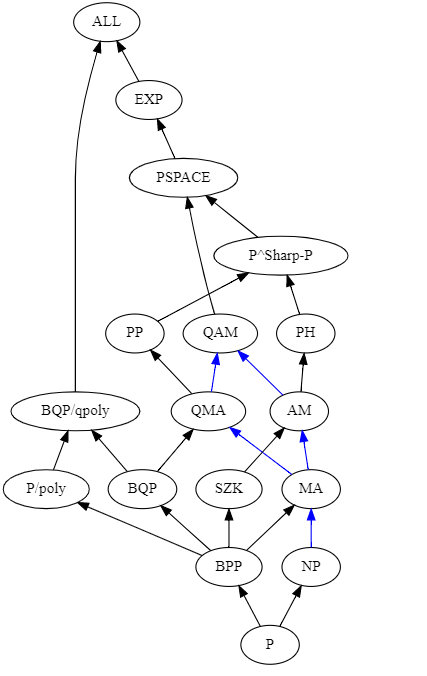
\includegraphics[width=4in]
  {simplified-graph-uncolored.png}}
  \caption{\label{fig:mini-zoo-inclusion} Inclusions that hold with respect to 
  every oracle for 17 complexity classes. Blue indicates that the lower class is 
  included in the upper class. Black indicates that the lower class and its 
  complement are included in the upper class.}
\end{figure}

\subsection{Oracle Separations and Collapses}

Now we present some of the inclusions that fail for some oracle, as well as some 
inclusions that do not relativize. As far as relativizing inclusions are 
concerned, the picture presented in Figure \ref{fig:mini-zoo-inclusion} is 
complete for the 17 complexity classes shown. We cannot, for instance, show that 
$\sP/\poly$ is contained in $\msf{BQP}$ or that $\msf{EXP}$ is contained in $\sP$
for every oracle. These particular examples hold for every oracle: in the former 
case because $\msf{BQP}$ is countable while $\sP/\poly$ is not, and in the latter
case because of the \textit{time-hierarchy theorem}.

For functions $f,g:\N\ra\N$, we write $f(n)=o(g(n))$ if $f(n)/g(n)\ra 0$ as 
$n\ra\infty$. Denote by $\msf{DTIME}(T(n))$ the class of languages that are 
computable in $T(n)$-time.

\begin{theorem}[Time-hierarchy theorem]
If $f,g:\N\ra\N$ satisfy $f(n)\log f(n)=o(g(n))$, then
\[
\msf{DTIME}(f(n))\subsetneq\msf{DTIME}(g(n))
\]
with respect to every oracle.
\end{theorem}
\begin{proof}
The technique used to prove this theorem is \textit{diagonalization}, inspired by
the set theoretic method of the same name. Since $g(n)$ grows much faster than 
$f(n)\log f(n)$, we have that $\msf{DTIME}(f(n))\subseteq\msf{DTIME}(g(n))$. It 
remains to show that $\msf{DTIME}(g(n))\not\subseteq\msf{DTIME}(f(n))$.

Let $U$ indicate the universal Turing machine of Theorem \ref{universal-machine}.
We carry out the following procedure: on input $x$, compute $M_x(x)$ on a 
suitable universal TM for $g(|x|)$ steps, where $M_x$ is the Turing machine 
encoded by $x$. If the computation finishes, output $1-M_x(x)$. Otherwise, output
$0$. Let $D$ be the Turing machine that follows this algorithm. By the choice of 
universal Turing machine and the fact that $f(n)\log f(n)=o(g(n))$, we have 
$D\in\msf{DTIME}(g(n))$.

Next, assume the language determined by $D$ lies in  $\msf{DTIME}(f(n))$. Then, 
there exists a Turing $M$ that decides the same language in $\Oh(f(n))$-time. Then
$M$ has some encoding, and in fact can be assumed to have infinitely many 
encodings, so we fix some encoding $y$ that is long enough so that $f(|y|)\log 
f(|y|)$ is much less than $g(|y|)$. Then the universal Turing machine can simulate
$M_y$ on input $y$ within $g(|y|)$ steps, and so $D(y)=1-M_y(y)=1-M(y)$, 
contradicting the assumption that $D(y)=M(y)$. Therefore, 
$\msf{DTIME}(g(n))\not\subseteq\msf{DTIME}(f(n))$.
\end{proof}

The time-hierarchy theorem proves that there is no oracle collapse from 
$\msf{EXP}$ to $\sP$. There is, however, an oracle collapse from $\msf{PSPACE}$ to
$\sP$; i.e., there is an oracle relative to which $\sP=\msf{PSPACE}$. The usual 
method to make use of a $\msf{PSPACE}$-complete problem---a language $\cL$ in 
$\msf{PSPACE}$ such that every other question in $\msf{PSPACE}$ can be reduced to 
the question of whether $y\in\cL$, where $y$ can be computed from the input in 
polynomial time. Then an oracle for $\cL$ does not give $\msf{PSPACE}$ any 
additional computational power, while boosting $\sP$ up to $\msf{PSPACE}$. 
However, in Section \ref{ah-plo-subsection} we will show that 
there is an even larger class that collapses to $\sP$.

Such a collapse also shows that there is an oracle relative to which $\sP=\NP$. 
There is also an oracle relative to which $\sP\neq\NP$, which establishes that no 
relativizing proof can settle the $\sP$ versus $\NP$ question. A \textit{password oracle} is a type of oracle $f$ constructed so that
$\sC_1^f\not\subseteq\sC_2^f$. Typically, $f$ is a function
$\Sigma^*\times\Sigma^*\rightarrow\Sigma^*$ chosen so that
$PW_f=\{x\in\Sigma:P\}$ lies in $\sC_1^f$ but not in $\sC_2^f$, where $P$ is a
proposition depending on the values of $f(x,y)$ for $y\in\Sigma^*$ (the
\textit{passwords} of $x$). The oracle $f$ can be adversarially constructed or,
in many cases, selected according to a random process.

\begin{theorem}
Let $f:\Sigma^{2*}\ra\Sigma\cup\{\square\}$ be a function selected randomly
according to the following rules:
\begin{itemize}
\item For every $x\in\Sigma^n$, there exists a unique $y\in\Sigma^n$ such that
$f(x,y)\neq\square$. This $y$ is selected using the uniform distribution on
$\Sigma^n$.
\item  For every $x\in\Sigma^n$, if $y$ is the unique element of $\Sigma^n$ such
that $f(x,y)\neq\square$, then $\Pr[f(x,y)=1]=\Pr[f(x,y)=0]=1/2$.
\end{itemize}
Then $(\cocap\cdot\msf{NP})^f\not\subseteq(\sP/\poly)^f$ with probability 1.
\end{theorem}

\begin{proof}
For each $x\in\Sigma^*$, define $PW_f(x)=f(x,y)$, where $y$ is the unique
element of $\Sigma^{|x|}$ such that $f(x,y)\neq\square$. Then
$PW_f\in(\cocap\cdot\msf{NP})^f$, because for a given $x\in\Sigma^*$ the unique
$y$ can be used as the certificate to check that $PW_f(x)=1$ or $PW_f(x)=0$.

Fix an enumeration $\{M_k\}$ of Turing machines. For $M_k$ and input of length
$n$, we allow computation times up to $C_kn^{r_k}$ and advice strings up to
length $D_kn^{s_k}$, where the coefficients and exponents are unbounded and
increasing as functions of $k$. Then, since for any $x\in\Sigma^n$ there are
$2^n$ possible values of $y$, while advice and computation time are polynomials
of $n$, we have
\[
\Pr[(\forall n)(\exists\text{ advice }a)(\forall|x|=n)[M_k(x,a)=PW_f(x)]]=0.
\]
\end{proof}

The above proof actually establishes the stronger claim that 
$(\cocap\cdot\msf{UP})^f\not\subseteq(\sP/\poly)^f$, where $\msf{UP}$ denotes 
\textit{unambiguous polynomial time} (see Subsection \ref{up-section}).